\chapter{O Projeto}

Esse capítulo descreverá a aplicação que foi desenvolvida para a realização dos testes, qual a arquitetura que foi utilizada no projeto, além de descrever os planos de testes.


\section{A Aplicação}

Para a execução dos testes de performance foi desenvolvido um Web service com as principais operações necessárias para manter os dados do AFD. O objetivo central da aplicação é manter os documentos da pasta funcional dos servidores. Como a aplicação deve armazenar aquivos, escolhemos gravar o arquivo no sistema operacional e armazenar o caminho para ele na base de dados. Na figura \ref{fig:ucmodel} temos o modelo de casos de uso e na figura \ref{fig:classmodel} temos uma breve descrição dos métodos do Web service. O objetivo ao se escolher realizar os testes de performance via Web service foi o de flexibilizar ao máximo as implementações em diversos bancos de dados. Na tabela \ref{tab:funcionalidades} a descrição das funcionalidades implementadas.

	\begin{figure}[!htbp]
		\begin{center}
			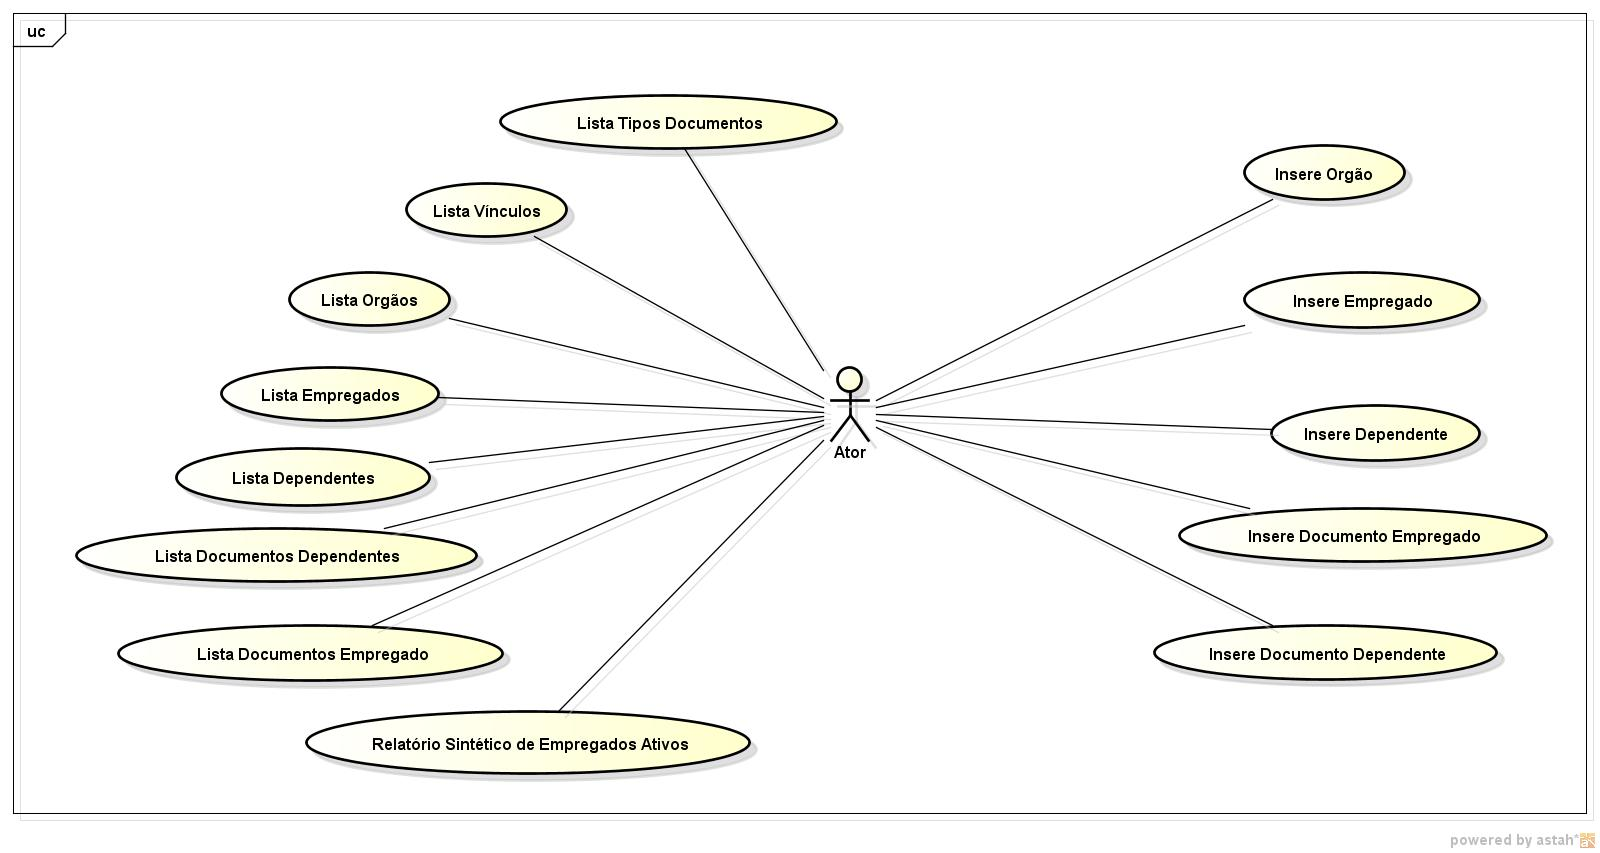
\includegraphics[width=1\textwidth]{diagrama_geral}
		\end{center}
		\caption{Modelo de Casos de Uso}
		\label{fig:ucmodel}
	\end{figure}

	\begin{figure}[!htbp]
		\begin{center}
			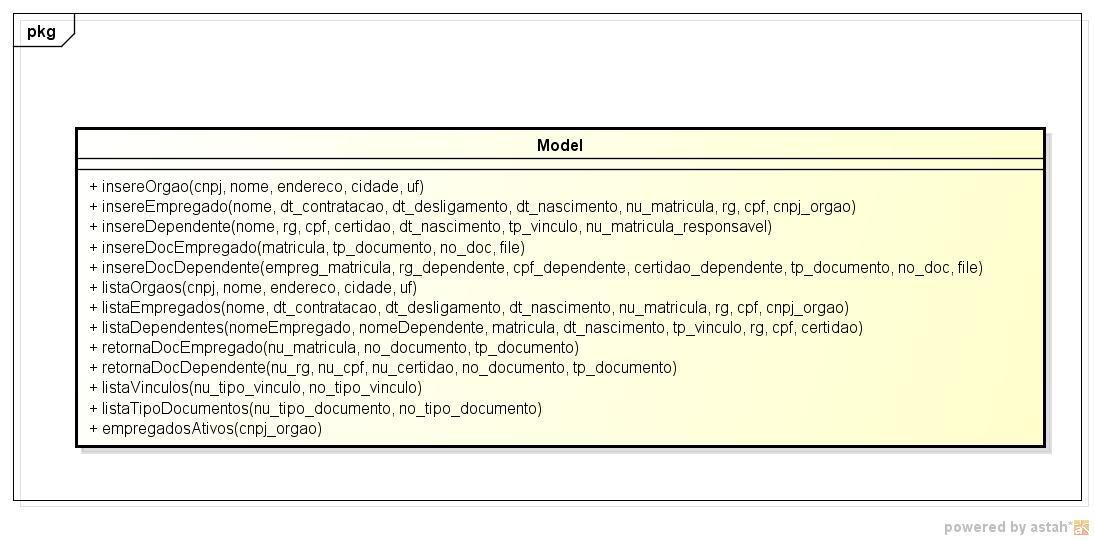
\includegraphics[width=1\textwidth]{class_model}
		\end{center}
		\caption{Descrição dos Métodos}
		\label{fig:classmodel}
	\end{figure}

\renewcommand{\arraystretch}{3}

\begin{table}
	\caption{Descrição das Funcionalidades}
	\begin{center}
	\begin{tabularx}{\textwidth}{ | c | X | }
		\hline
			\textbf{Funcionalidade} & \multicolumn{1}{c|}{\textbf{Descrição}} \\
		\hline
			Insere Orgão & \noindent\parbox[c]{\hsize}{Permite inserir as unidades pagadoras ou orgãos que terão os dados dos empregados mantidos no sistema.} \\
		\hline
			Insere Empregado & \noindent\parbox[c]{\hsize}{Permite inserir os empregados de cada orgão.} \\
		\hline
			Insere Dependente & \noindent\parbox[c]{\hsize}{Permite inserir os dependentes de cada empregado.}\\
		\hline
			Insere Documento Dependente & \noindent\parbox[c]{\hsize}{Permite inserir os documentos dos dependentes que farão parte da pasta funcional do empregado.} \\
		\hline
			Insere Documento Empregado & \noindent\parbox[c]{\hsize}{Permite inserir os documentos que farão parte da pasta funcional do empregado.} \\
		\hline
			Lista Orgãos & \noindent\parbox[c]{\hsize}{Lista os dados dos órgãos cadastrados no sistema.} \\
		\hline
			Lista Empregados & \noindent\parbox[c]{\hsize}{Lista os dados dos empregados cadastrados no sistema.} \\
		\hline
			Lista Dependentes & \noindent\parbox[c]{\hsize}{Lista os dados dos dependentes dos empregados.} \\
		\hline
			Lista Documentos Empregados & \noindent\parbox[c]{\hsize}{Retorna os documentos da pasta funcional do empregado.} \\
		\hline
			Lista Documentos Dependentes & \noindent\parbox[c]{\hsize}{Retorna os documentos dos dependentes dos empregados.} \\
		\hline
			Relatório Sintético de Empregados Ativos & \noindent\parbox[c]{\hsize}{Calcula e exibe a quantidade de empregados ativos por orgão.} \\
		\hline
			Lista Vínculos & \noindent\parbox[c]{\hsize}{Lista os valores possíveis para os tipos de vínculos entre empregados e dependentes.} \\
		\hline
			Lista Tipo Documentos & \noindent\parbox[c]{\hsize}{Lista os valores possíveis para os tipos de documentos.} \\
		\hline
	\end {tabularx}
	\end{center}
	%\caption{Fonte: http://docs.mongodb.org}
	\label{tab:funcionalidades}
\end{table}

\section{A Arquitetura do Projeto}

Para cumprirmos o nosso objetivo, que é testar a nossa aplicação com diferentes bancos de dados, montamos uma arquitetura simples, mas que nos permitisse trocar as implementações da camada de persistência sem maiores esforços. Para a execução dos testes utilizamos o JMeter. A aplicação foi desenvolvida em python com o apoio do framework web2py na implementação do Web service. A linguagem de programação python foi escolhida pela facilidade de encontrar drivers de diversos bancos de dados relacionais e não relacionais, além de ser uma linguagem orientada a objetos e de ampla utilização. O framework web2py foi adicionado ao projeto pelo motivo de suportar a implementação de Web services de modo rápido e fácil, altém da geração automática do WSDL (arquivo que contém a descrição das operações do Web service). A diagramação da arquitetura pode ser vista na figura \ref{fig:arquitetura}

	\begin{figure}[!htbp]
		\begin{center}
			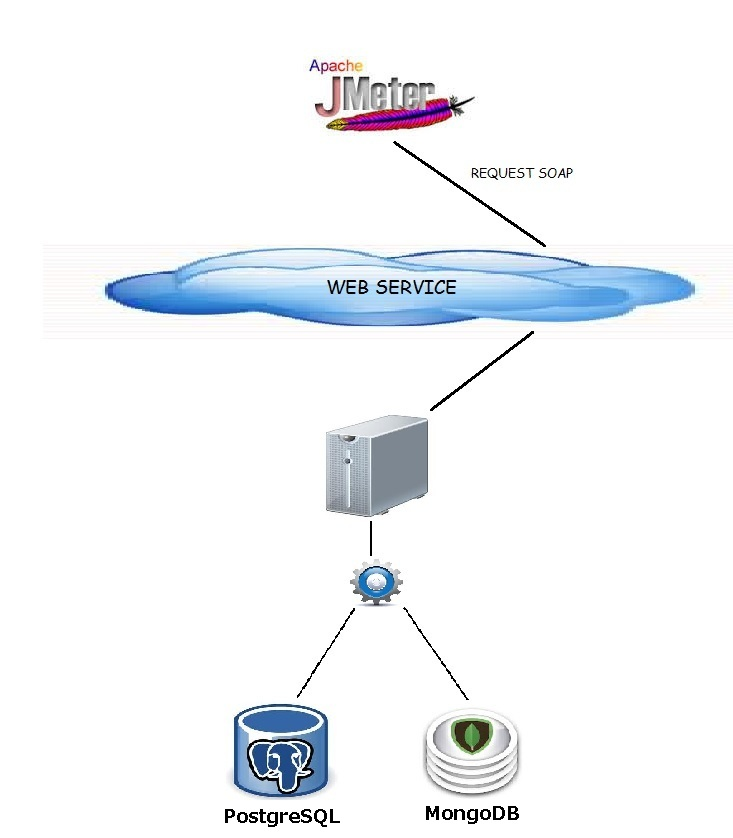
\includegraphics[width=0.5\textwidth]{arquitetura}
		\end{center}
		\caption{Arquitetura de Testes}
		\label{fig:arquitetura}
	\end{figure}

\subsection{web2py}

Web2py é um framework para desenvolvimento ágil de aplicações web, software livre e gratuito. Ele é escrito e programável em Python. [http://www.web2py.com/] web2py foi inspirado pelo Ruby on Rails e Django. Tem seu foco no desenvolvimento ágil e segue o MVC (Model View Controller). Toda aplicação web2py é composta por Models (arquivos que contem a descrição dos dados), Views (arquivos que contem a descrição dos dados que serão apresentados), Controlers (arquivos que contem a lógica e workflow do negócio), Cron Jobs (tarefas que precisam ser executadas regularmente) e Static Files (imagens, scripts, folhas de estilos, etc.)

Quando se trata de Web services, web2py oferece suporte para diversos protocolos, incluindo XML, JSON, RSS,CSV,XMLRPC,JSONRPC,AMFRPC, e SOAP.  O web2py inclui um cliente e servidor SOAP (pysimplesoap) criado por Mariano Reingart. Uma facilidade encontrada é a geração automática do WSDL e a pagina com a descrição dos métodos.

\section{Os Planos de Teste}

Foi desenvolvido um plano de testes no JMeter para cada funcionalidade da nossa aplicação. O testador utilizado no nosso projeto foi o de Requisição SOAP/XML - RPC. É nele que configuramos as requisições que serão feitas ao Web service da aplicação. Além de configurar uma requisição para cada plano de teste, temos como parametrizar outras configurações como a quantidade de usuários virtuais e o intervalo entre a inicialização de cada usuário. Na tabela \ref{tab:configplanoteste} temos as principais configurações dos nossos planos de teste. Os planos de testes desenvolvidos são basicamente de dois tipos: inserção e consulta. Sendo assim, os passos que eles executam são os mesmos.

\begin{table}
	\caption{Principais configurações dos Planos de Teste}
	\begin{center}
	\begin{tabularx}{\textwidth}{ | c | X | }
	\hline
		\textbf{Parâmetro} & \multicolumn{1}{c|}{\textbf{Descrição}} \\
	\hline
		Quantidade de usuários virtuais (threads) & Quanto maior o número de usuários virtuais, maior será o número de requisições simultâneas que a nossa aplicação terá que responder.\\
	\hline 
		Tempo de inicialização dos usuários virtuais & Indica o tempo total para a inicialização de todos os usuários virtuais. Para encontrarmos o tempo entre a inicialização de cada usuário devemos dividir pelo total de usuários virtuais.\\
	\hline
		O local dos arquivos CSV & Esses arquivos devem ser gerados antes do início dos testes com o apóio de um script.\\
	\hline
		Intervalo de medição dos gráficos & É o intervalo de tempo em que o JMeter faz as medidas para plotar cada gráfico.\\
	\hline
	\end {tabularx}
	\end{center}
	\label{tab:configplanoteste}
\end{table}

\subsection{Planos de Teste de Inserção}

Os planos de Testes de Inserção executam os seguintes passos:

\begin{enumerate}
\item Configuração de Dados CSV - É indicado onde está o arquivo csv de onde as threads lerão os valores a serem enviados na requisição soap;
\item Requisição SOAP/XML-RPC - É configurada a URL do Web service e a requisição que será realizada. Cada requisição será montada com os dados lidos do arquivo csv. Cada thread lê uma linha diferente do arquivo.
\item Gráfico de Tempo de Resposta -  Elemento responsável por gerar um gráfico a partir dos dados da requisição feita. O gráfico exibe a  evolução do tempo de resposta das requisições feitas.
\item Gráfico de Resultados - Elemento responsável por exibir a evolução dos tempos das requisições, a média dos tempos das requisições, a derivação do tempo das requisições e a vazão.
\end{enumerate}

\subsection{Planos de Teste de Consulta}

Os planos de Testes de Consulta executam os seguintes passos:

\begin{enumerate}
\item Requisição SOAP/XML-RPC - É configurada a URL do Web service e a requisição que será realizada. Cada requisição será montada com os dados lidos do arquivo csv. Cada thread lê uma linha diferente do arquivo.
\item Gráfico de Tempo de Resposta -  Elemento responsável por gerar um gráfico a partir dos dados da requisição feita. O gráfico exibe a  evolução do tempo de resposta das requisições feitas.
\item Gráfico de Resultados - Elemento responsável por exibir a evolução dos tempos das requisições, a média dos tempos das requisições, a derivação do tempo das requisições e a vazão.
\end{enumerate}


\chapter {Execução dos Testes}

Nesse capítulo vamos descrever o ambiente onde os testes foram realizados, as métricas que foram escolhidas para medir a performance e os resultados obtidos.

\section{Ambiente de testes}

Os testes foram realizados em uma máquina virtualizada, via VirtualBox, com as seguintes configurações:

\begin{itemize}
\item Sistema Operacional: Debian GNU/Linux 6.0
\item Quantidade de Processadores: 1 
\item Quantidade de Memória RAM: 2048 MB
\item Capacidade do HD: 60 GB
\item Mongo DB: Versão 2.4.0 com configurações padrão
\item PostgreSQL: Versão 8.4.16
\end{itemize}

\section{Massa de Dados}

Conforme Molyneaux diz ~\cite{theartoftestperf}, a importância de prover a quantidade de dados de qualidade para um teste não pode ser exagerada. Segundo ele a quantidade e a qualidade dos dados podem definir o sucesso ou insucesso dos testes. Para o nosso projeto foi desenvolvido um script em python para a geração da massa de dados. Os dados podem tanto ser inseridos diretamente na base de dados quanto em arquivos CSV que serão utilizados durante os testes. Os arquivos utilizados nos testes possuem tamanho médio de 400 KB. A quantidade de dados gerados também pode ser configurada pelo seguinte:

\begin{enumerate}
	\item Quantidade de Unidades Pagadoras (Orgãos);
	\item Quantidade de empregados por orgão;
	\item Quantidade de dependentes por empregado;
	\item Quantidade de documentos por empregado;
	\item Quantidade de documentos por dependente;
\end{enumerate}

\section{Métricas}

Quando se quer balancear o custo e a performance, todos os envolvidos na produção do software se preocupam com a execução de testes de performance. A avaliação de performance é necessária em todas as etapas do ciclo de vida de software e é requerida sempre que o arquiteto precisa comparar alternativasv~\cite{rajjain}. Em um teste de performance a escolha das métricas é de grande importância. Segundo Raj Jain ~\cite{rajjain}, escolher as métricas erradas é um dos erros mais comuns. Para o nosso trabalho as métricas escolhidas foram a vazão e o tempo de resposta.

\section{Resultados}



